\documentclass[1p]{elsarticle_modified}
%\bibliographystyle{elsarticle-num}

%\usepackage[colorlinks]{hyperref}
%\usepackage{abbrmath_seonhwa} %\Abb, \Ascr, \Acal ,\Abf, \Afrak
\usepackage{amsfonts}
\usepackage{amssymb}
\usepackage{amsmath}
\usepackage{amsthm}
\usepackage{scalefnt}
\usepackage{amsbsy}
\usepackage{kotex}
\usepackage{caption}
\usepackage{subfig}
\usepackage{color}
\usepackage{graphicx}
\usepackage{xcolor} %% white, black, red, green, blue, cyan, magenta, yellow
\usepackage{float}
\usepackage{setspace}
\usepackage{hyperref}

\usepackage{tikz}
\usetikzlibrary{arrows}

\usepackage{multirow}
\usepackage{array} % fixed length table
\usepackage{hhline}

%%%%%%%%%%%%%%%%%%%%%
\makeatletter
\renewcommand*\env@matrix[1][\arraystretch]{%
	\edef\arraystretch{#1}%
	\hskip -\arraycolsep
	\let\@ifnextchar\new@ifnextchar
	\array{*\c@MaxMatrixCols c}}
\makeatother %https://tex.stackexchange.com/questions/14071/how-can-i-increase-the-line-spacing-in-a-matrix
%%%%%%%%%%%%%%%

\usepackage[normalem]{ulem}

\newcommand{\msout}[1]{\ifmmode\text{\sout{\ensuremath{#1}}}\else\sout{#1}\fi}
%SOURCE: \msout is \stkout macro in https://tex.stackexchange.com/questions/20609/strikeout-in-math-mode

\newcommand{\cancel}[1]{
	\ifmmode
	{\color{red}\msout{#1}}
	\else
	{\color{red}\sout{#1}}
	\fi
}

\newcommand{\add}[1]{
	{\color{blue}\uwave{#1}}
}

\newcommand{\replace}[2]{
	\ifmmode
	{\color{red}\msout{#1}}{\color{blue}\uwave{#2}}
	\else
	{\color{red}\sout{#1}}{\color{blue}\uwave{#2}}
	\fi
}

\newcommand{\Sol}{\mathcal{S}} %segment
\newcommand{\D}{D} %diagram
\newcommand{\A}{\mathcal{A}} %arc


%%%%%%%%%%%%%%%%%%%%%%%%%%%%%5 test

\def\sl{\operatorname{\textup{SL}}(2,\Cbb)}
\def\psl{\operatorname{\textup{PSL}}(2,\Cbb)}
\def\quan{\mkern 1mu \triangleright \mkern 1mu}

\theoremstyle{definition}
\newtheorem{thm}{Theorem}[section]
\newtheorem{prop}[thm]{Proposition}
\newtheorem{lem}[thm]{Lemma}
\newtheorem{ques}[thm]{Question}
\newtheorem{cor}[thm]{Corollary}
\newtheorem{defn}[thm]{Definition}
\newtheorem{exam}[thm]{Example}
\newtheorem{rmk}[thm]{Remark}
\newtheorem{alg}[thm]{Algorithm}

\newcommand{\I}{\sqrt{-1}}
\begin{document}

%\begin{frontmatter}
%
%\title{Boundary parabolic representations of knots up to 8 crossings}
%
%%% Group authors per affiliation:
%\author{Yunhi Cho} 
%\address{Department of Mathematics, University of Seoul, Seoul, Korea}
%\ead{yhcho@uos.ac.kr}
%
%
%\author{Seonhwa Kim} %\fnref{s_kim}}
%\address{Center for Geometry and Physics, Institute for Basic Science, Pohang, 37673, Korea}
%\ead{ryeona17@ibs.re.kr}
%
%\author{Hyuk Kim}
%\address{Department of Mathematical Sciences, Seoul National University, Seoul 08826, Korea}
%\ead{hyukkim@snu.ac.kr}
%
%\author{Seokbeom Yoon}
%\address{Department of Mathematical Sciences, Seoul National University, Seoul, 08826,  Korea}
%\ead{sbyoon15@snu.ac.kr}
%
%\begin{abstract}
%We find all boundary parabolic representation of knots up to 8 crossings.
%
%\end{abstract}
%\begin{keyword}
%    \MSC[2010] 57M25 
%\end{keyword}
%
%\end{frontmatter}

%\linenumbers
%\tableofcontents
%
\newcommand\colored[1]{\textcolor{white}{\rule[-0.35ex]{0.8em}{1.4ex}}\kern-0.8em\color{red} #1}%
%\newcommand\colored[1]{\textcolor{white}{ #1}\kern-2.17ex	\textcolor{white}{ #1}\kern-1.81ex	\textcolor{white}{ #1}\kern-2.15ex\color{red}#1	}

{\Large $\underline{12a_{0378}~(K12a_{0378})}$}

\setlength{\tabcolsep}{10pt}
\renewcommand{\arraystretch}{1.6}
\vspace{1cm}\begin{tabular}{m{100pt}>{\centering\arraybackslash}m{274pt}}
\multirow{5}{120pt}{
	\centering
	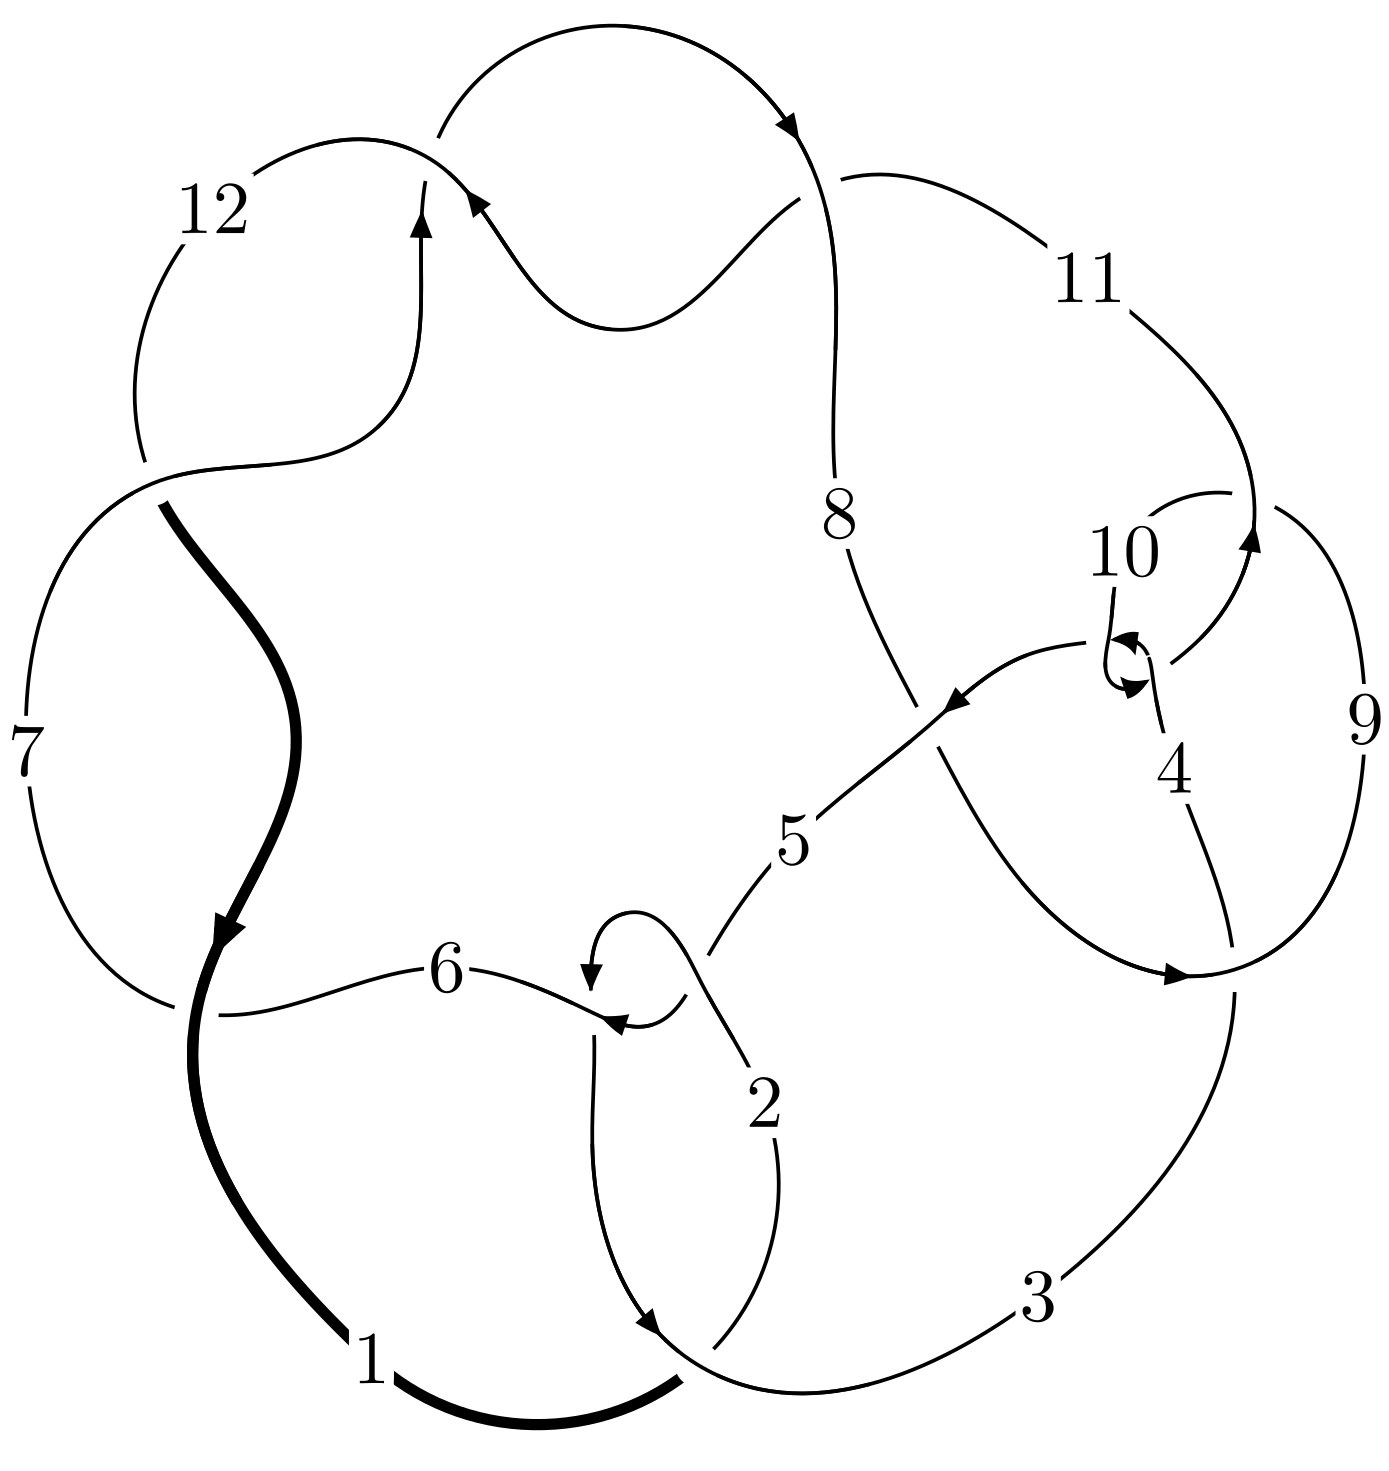
\includegraphics[width=112pt]{../../../GIT/diagram.site/Diagrams/png/1179_12a_0378.png}\\
\ \ \ A knot diagram\footnotemark}&
\allowdisplaybreaks
\textbf{Linearized knot diagam} \\
\cline{2-2}
 &
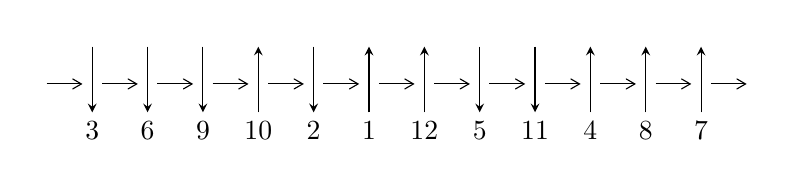
\begin{tikzpicture}[x=20pt, y=17pt]
	% nodes
	\node (C0) at (0, 0) {};
	\node (C1) at (1, 0) {};
	\node (C1U) at (1, +1) {};
	\node (C1D) at (1, -1) {3};

	\node (C2) at (2, 0) {};
	\node (C2U) at (2, +1) {};
	\node (C2D) at (2, -1) {6};

	\node (C3) at (3, 0) {};
	\node (C3U) at (3, +1) {};
	\node (C3D) at (3, -1) {9};

	\node (C4) at (4, 0) {};
	\node (C4U) at (4, +1) {};
	\node (C4D) at (4, -1) {10};

	\node (C5) at (5, 0) {};
	\node (C5U) at (5, +1) {};
	\node (C5D) at (5, -1) {2};

	\node (C6) at (6, 0) {};
	\node (C6U) at (6, +1) {};
	\node (C6D) at (6, -1) {1};

	\node (C7) at (7, 0) {};
	\node (C7U) at (7, +1) {};
	\node (C7D) at (7, -1) {12};

	\node (C8) at (8, 0) {};
	\node (C8U) at (8, +1) {};
	\node (C8D) at (8, -1) {5};

	\node (C9) at (9, 0) {};
	\node (C9U) at (9, +1) {};
	\node (C9D) at (9, -1) {11};

	\node (C10) at (10, 0) {};
	\node (C10U) at (10, +1) {};
	\node (C10D) at (10, -1) {4};

	\node (C11) at (11, 0) {};
	\node (C11U) at (11, +1) {};
	\node (C11D) at (11, -1) {8};

	\node (C12) at (12, 0) {};
	\node (C12U) at (12, +1) {};
	\node (C12D) at (12, -1) {7};
	\node (C13) at (13, 0) {};

	% arrows
	\draw[->,>={angle 60}]
	(C0) edge (C1) (C1) edge (C2) (C2) edge (C3) (C3) edge (C4) (C4) edge (C5) (C5) edge (C6) (C6) edge (C7) (C7) edge (C8) (C8) edge (C9) (C9) edge (C10) (C10) edge (C11) (C11) edge (C12) (C12) edge (C13) ;	\draw[->,>=stealth]
	(C1U) edge (C1D) (C2U) edge (C2D) (C3U) edge (C3D) (C4D) edge (C4U) (C5U) edge (C5D) (C6D) edge (C6U) (C7D) edge (C7U) (C8U) edge (C8D) (C9U) edge (C9D) (C10D) edge (C10U) (C11D) edge (C11U) (C12D) edge (C12U) ;
	\end{tikzpicture} \\
\hhline{~~} \\& 
\textbf{Solving Sequence} \\ \cline{2-2} 
 &
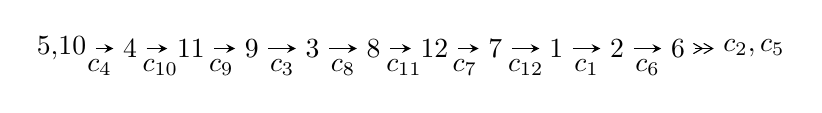
\begin{tikzpicture}[x=22pt, y=7pt]
	% node
	\node (A0) at (-1/8, 0) {5,10};
	\node (A1) at (1, 0) {4};
	\node (A2) at (2, 0) {11};
	\node (A3) at (3, 0) {9};
	\node (A4) at (4, 0) {3};
	\node (A5) at (5, 0) {8};
	\node (A6) at (6, 0) {12};
	\node (A7) at (7, 0) {7};
	\node (A8) at (8, 0) {1};
	\node (A9) at (9, 0) {2};
	\node (A10) at (10, 0) {6};
	\node (C1) at (1/2, -1) {$c_{4}$};
	\node (C2) at (3/2, -1) {$c_{10}$};
	\node (C3) at (5/2, -1) {$c_{9}$};
	\node (C4) at (7/2, -1) {$c_{3}$};
	\node (C5) at (9/2, -1) {$c_{8}$};
	\node (C6) at (11/2, -1) {$c_{11}$};
	\node (C7) at (13/2, -1) {$c_{7}$};
	\node (C8) at (15/2, -1) {$c_{12}$};
	\node (C9) at (17/2, -1) {$c_{1}$};
	\node (C10) at (19/2, -1) {$c_{6}$};
	\node (A11) at (45/4, 0) {$c_{2},c_{5}$};

	% edge
	\draw[->,>=stealth]	
	(A0) edge (A1) (A1) edge (A2) (A2) edge (A3) (A3) edge (A4) (A4) edge (A5) (A5) edge (A6) (A6) edge (A7) (A7) edge (A8) (A8) edge (A9) (A9) edge (A10) ;
	\draw[->>,>={angle 60}]	
	(A10) edge (A11);
\end{tikzpicture} \\ 

\end{tabular} \\

\footnotetext{
The image of knot diagram is generated by the software ``\textbf{Draw programme}" developed by Andrew Bartholomew(\url{http://www.layer8.co.uk/maths/draw/index.htm\#Running-draw}), where we modified some parts for our purpose(\url{https://github.com/CATsTAILs/LinksPainter}).
}\phantom \\ \newline 
\centering \textbf{Ideals for irreducible components\footnotemark of $X_{\text{par}}$} 
 
\begin{align*}
I^u_{1}&=\langle 
u^{63}- u^{62}+\cdots+2 u-1\rangle \\
\\
\end{align*}
\raggedright * 1 irreducible components of $\dim_{\mathbb{C}}=0$, with total 63 representations.\\
\footnotetext{All coefficients of polynomials are rational numbers. But the coefficients are sometimes approximated in decimal forms when there is not enough margin.}
\newpage
\renewcommand{\arraystretch}{1}
\centering \section*{I. $I^u_{1}= \langle u^{63}- u^{62}+\cdots+2 u-1 \rangle$}
\flushleft \textbf{(i) Arc colorings}\\
\begin{tabular}{m{7pt} m{180pt} m{7pt} m{180pt} }
\flushright $a_{5}=$&$\begin{pmatrix}1\\0\end{pmatrix}$ \\
\flushright $a_{10}=$&$\begin{pmatrix}0\\u\end{pmatrix}$ \\
\flushright $a_{4}=$&$\begin{pmatrix}1\\u^2\end{pmatrix}$ \\
\flushright $a_{11}=$&$\begin{pmatrix}u\\u^3+u\end{pmatrix}$ \\
\flushright $a_{9}=$&$\begin{pmatrix}u^3\\u^5+u^3+u\end{pmatrix}$ \\
\flushright $a_{3}=$&$\begin{pmatrix}- u^6- u^4+1\\- u^8-2 u^6-2 u^4\end{pmatrix}$ \\
\flushright $a_{8}=$&$\begin{pmatrix}u^5+2 u^3+u\\u^5+u^3+u\end{pmatrix}$ \\
\flushright $a_{12}=$&$\begin{pmatrix}u^{13}+4 u^{11}+7 u^9+6 u^7+2 u^5+u\\u^{13}+3 u^{11}+5 u^9+4 u^7+2 u^5+u^3+u\end{pmatrix}$ \\
\flushright $a_{7}=$&$\begin{pmatrix}u^{21}+6 u^{19}+17 u^{17}+28 u^{15}+28 u^{13}+16 u^{11}+5 u^9+2 u^7+3 u^5+2 u^3+u\\u^{21}+5 u^{19}+13 u^{17}+20 u^{15}+20 u^{13}+13 u^{11}+7 u^9+4 u^7+3 u^5+u^3+u\end{pmatrix}$ \\
\flushright $a_{1}=$&$\begin{pmatrix}u^{29}+8 u^{27}+\cdots+4 u^5+u\\u^{29}+7 u^{27}+\cdots+u^3+u\end{pmatrix}$ \\
\flushright $a_{2}=$&$\begin{pmatrix}u^{43}+10 u^{41}+\cdots+6 u^7- u^3\\u^{45}+11 u^{43}+\cdots+u^3+u\end{pmatrix}$ \\
\flushright $a_{6}=$&$\begin{pmatrix}u^{37}+10 u^{35}+\cdots+2 u^3+u\\u^{37}+9 u^{35}+\cdots+u^3+u\end{pmatrix}$\\&\end{tabular}
\flushleft \textbf{(ii) Obstruction class $= -1$}\\~\\
\flushleft \textbf{(iii) Cusp Shapes $= 4 u^{61}-4 u^{60}+\cdots+4 u-6$}\\~\\
\newpage\renewcommand{\arraystretch}{1}
\flushleft \textbf{(iv) u-Polynomials at the component}\newline \\
\begin{tabular}{m{50pt}|m{274pt}}
Crossings & \hspace{64pt}u-Polynomials at each crossing \\
\hline $$\begin{aligned}c_{1}\end{aligned}$$&$\begin{aligned}
&u^{63}+37 u^{62}+\cdots+16 u^3+1
\end{aligned}$\\
\hline $$\begin{aligned}c_{2},c_{5}\end{aligned}$$&$\begin{aligned}
&u^{63}+u^{62}+\cdots+2 u+1
\end{aligned}$\\
\hline $$\begin{aligned}c_{3}\end{aligned}$$&$\begin{aligned}
&u^{63}- u^{62}+\cdots-386 u+317
\end{aligned}$\\
\hline $$\begin{aligned}c_{4},c_{10}\end{aligned}$$&$\begin{aligned}
&u^{63}+u^{62}+\cdots+2 u+1
\end{aligned}$\\
\hline $$\begin{aligned}c_{6},c_{7},c_{11}\\c_{12}\end{aligned}$$&$\begin{aligned}
&u^{63}+3 u^{62}+\cdots+16 u+1
\end{aligned}$\\
\hline $$\begin{aligned}c_{8}\end{aligned}$$&$\begin{aligned}
&u^{63}+5 u^{62}+\cdots+360 u+31
\end{aligned}$\\
\hline $$\begin{aligned}c_{9}\end{aligned}$$&$\begin{aligned}
&u^{63}+31 u^{62}+\cdots+16 u^3-1
\end{aligned}$\\
\hline
\end{tabular}\\~\\
\newpage\renewcommand{\arraystretch}{1}
\flushleft \textbf{(v) Riley Polynomials at the component}\newline \\
\begin{tabular}{m{50pt}|m{274pt}}
Crossings & \hspace{64pt}Riley Polynomials at each crossing \\
\hline $$\begin{aligned}c_{1}\end{aligned}$$&$\begin{aligned}
&y^{63}-21 y^{62}+\cdots-64 y^2-1
\end{aligned}$\\
\hline $$\begin{aligned}c_{2},c_{5}\end{aligned}$$&$\begin{aligned}
&y^{63}-37 y^{62}+\cdots+16 y^3-1
\end{aligned}$\\
\hline $$\begin{aligned}c_{3}\end{aligned}$$&$\begin{aligned}
&y^{63}-25 y^{62}+\cdots+1252156 y-100489
\end{aligned}$\\
\hline $$\begin{aligned}c_{4},c_{10}\end{aligned}$$&$\begin{aligned}
&y^{63}+31 y^{62}+\cdots+16 y^3-1
\end{aligned}$\\
\hline $$\begin{aligned}c_{6},c_{7},c_{11}\\c_{12}\end{aligned}$$&$\begin{aligned}
&y^{63}+79 y^{62}+\cdots-80 y-1
\end{aligned}$\\
\hline $$\begin{aligned}c_{8}\end{aligned}$$&$\begin{aligned}
&y^{63}-13 y^{62}+\cdots+27176 y-961
\end{aligned}$\\
\hline $$\begin{aligned}c_{9}\end{aligned}$$&$\begin{aligned}
&y^{63}+3 y^{62}+\cdots+128 y^2-1
\end{aligned}$\\
\hline
\end{tabular}\\~\\
\newpage\flushleft \textbf{(vi) Complex Volumes and Cusp Shapes}
$$\begin{array}{c|c|c}  
\text{Solutions to }I^u_{1}& \I (\text{vol} + \sqrt{-1}CS) & \text{Cusp shape}\\
 \hline 
\begin{aligned}
u &= -0.621935 + 0.782730 I\end{aligned}
 & -9.96990 + 2.39006 I & -4.17438 + 0. I\phantom{ +0.000000I} \\ \hline\begin{aligned}
u &= -0.621935 - 0.782730 I\end{aligned}
 & -9.96990 - 2.39006 I & -4.17438 + 0. I\phantom{ +0.000000I} \\ \hline\begin{aligned}
u &= \phantom{-}0.438527 + 0.907377 I\end{aligned}
 & -1.96094 - 0.80799 I & -3.24469 + 2.24299 I \\ \hline\begin{aligned}
u &= \phantom{-}0.438527 - 0.907377 I\end{aligned}
 & -1.96094 + 0.80799 I & -3.24469 - 2.24299 I \\ \hline\begin{aligned}
u &= -0.630886 + 0.761128 I\end{aligned}
 & -9.90322 - 7.24194 I & -3.95069 + 6.24276 I \\ \hline\begin{aligned}
u &= -0.630886 - 0.761128 I\end{aligned}
 & -9.90322 + 7.24194 I & -3.95069 - 6.24276 I \\ \hline\begin{aligned}
u &= \phantom{-}0.618288 + 0.768075 I\end{aligned}
 & -6.12298 + 2.40025 I & -0.83833 - 3.23354 I \\ \hline\begin{aligned}
u &= \phantom{-}0.618288 - 0.768075 I\end{aligned}
 & -6.12298 - 2.40025 I & -0.83833 + 3.23354 I \\ \hline\begin{aligned}
u &= -0.473047 + 1.008350 I\end{aligned}
 & -0.44679 - 2.73565 I & \phantom{-0.000000 } 0 \\ \hline\begin{aligned}
u &= -0.473047 - 1.008350 I\end{aligned}
 & -0.44679 + 2.73565 I & \phantom{-0.000000 } 0 \\ \hline\begin{aligned}
u &= \phantom{-}0.309687 + 1.086540 I\end{aligned}
 & -4.07179 + 0.35561 I & \phantom{-0.000000 } 0 \\ \hline\begin{aligned}
u &= \phantom{-}0.309687 - 1.086540 I\end{aligned}
 & -4.07179 - 0.35561 I & \phantom{-0.000000 } 0 \\ \hline\begin{aligned}
u &= \phantom{-}0.281866 + 0.810813 I\end{aligned}
 & -2.03136 - 0.82581 I & -5.70235 + 1.89666 I \\ \hline\begin{aligned}
u &= \phantom{-}0.281866 - 0.810813 I\end{aligned}
 & -2.03136 + 0.82581 I & -5.70235 - 1.89666 I \\ \hline\begin{aligned}
u &= \phantom{-}0.563966 + 0.645928 I\end{aligned}
 & -1.23878 + 4.99873 I & -1.02686 - 8.32445 I \\ \hline\begin{aligned}
u &= \phantom{-}0.563966 - 0.645928 I\end{aligned}
 & -1.23878 - 4.99873 I & -1.02686 + 8.32445 I \\ \hline\begin{aligned}
u &= -0.274490 + 1.109110 I\end{aligned}
 & -6.89845 + 3.68623 I & \phantom{-0.000000 } 0 \\ \hline\begin{aligned}
u &= -0.274490 - 1.109110 I\end{aligned}
 & -6.89845 - 3.68623 I & \phantom{-0.000000 } 0 \\ \hline\begin{aligned}
u &= -0.512226 + 1.042810 I\end{aligned}
 & \phantom{-}0.00316 - 3.27794 I & \phantom{-0.000000 } 0 \\ \hline\begin{aligned}
u &= -0.512226 - 1.042810 I\end{aligned}
 & \phantom{-}0.00316 + 3.27794 I & \phantom{-0.000000 } 0 \\ \hline\begin{aligned}
u &= \phantom{-}0.795174 + 0.261887 I\end{aligned}
 & -12.4090 - 9.0599 I & -4.87131 + 5.08954 I \\ \hline\begin{aligned}
u &= \phantom{-}0.795174 - 0.261887 I\end{aligned}
 & -12.4090 + 9.0599 I & -4.87131 - 5.08954 I \\ \hline\begin{aligned}
u &= \phantom{-}0.792169 + 0.247301 I\end{aligned}
 & -12.62010 + 0.73676 I & -5.26880 - 0.86219 I \\ \hline\begin{aligned}
u &= \phantom{-}0.792169 - 0.247301 I\end{aligned}
 & -12.62010 - 0.73676 I & -5.26880 + 0.86219 I \\ \hline\begin{aligned}
u &= -0.788814 + 0.256117 I\end{aligned}
 & -8.63854 + 4.09024 I & -1.84772 - 2.15081 I \\ \hline\begin{aligned}
u &= -0.788814 - 0.256117 I\end{aligned}
 & -8.63854 - 4.09024 I & -1.84772 + 2.15081 I \\ \hline\begin{aligned}
u &= -0.335883 + 1.123950 I\end{aligned}
 & -7.59429 - 3.78030 I & \phantom{-0.000000 } 0 \\ \hline\begin{aligned}
u &= -0.335883 - 1.123950 I\end{aligned}
 & -7.59429 + 3.78030 I & \phantom{-0.000000 } 0 \\ \hline\begin{aligned}
u &= \phantom{-}0.444654 + 1.090310 I\end{aligned}
 & -4.15081 + 3.62964 I & \phantom{-0.000000 } 0 \\ \hline\begin{aligned}
u &= \phantom{-}0.444654 - 1.090310 I\end{aligned}
 & -4.15081 - 3.62964 I & \phantom{-0.000000 } 0\\
 \hline 
 \end{array}$$\newpage$$\begin{array}{c|c|c}  
\text{Solutions to }I^u_{1}& \I (\text{vol} + \sqrt{-1}CS) & \text{Cusp shape}\\
 \hline 
\begin{aligned}
u &= \phantom{-}0.530104 + 1.071360 I\end{aligned}
 & -0.56847 + 7.03450 I & \phantom{-0.000000 } 0 \\ \hline\begin{aligned}
u &= \phantom{-}0.530104 - 1.071360 I\end{aligned}
 & -0.56847 - 7.03450 I & \phantom{-0.000000 } 0 \\ \hline\begin{aligned}
u &= -0.286256 + 1.181430 I\end{aligned}
 & -13.08250 + 0.76656 I & \phantom{-0.000000 } 0 \\ \hline\begin{aligned}
u &= -0.286256 - 1.181430 I\end{aligned}
 & -13.08250 - 0.76656 I & \phantom{-0.000000 } 0 \\ \hline\begin{aligned}
u &= \phantom{-}0.280566 + 1.184730 I\end{aligned}
 & -16.9082 - 5.7443 I & \phantom{-0.000000 } 0 \\ \hline\begin{aligned}
u &= \phantom{-}0.280566 - 1.184730 I\end{aligned}
 & -16.9082 + 5.7443 I & \phantom{-0.000000 } 0 \\ \hline\begin{aligned}
u &= -0.720190 + 0.301321 I\end{aligned}
 & -2.72172 + 6.49499 I & -2.54742 - 7.00667 I \\ \hline\begin{aligned}
u &= -0.720190 - 0.301321 I\end{aligned}
 & -2.72172 - 6.49499 I & -2.54742 + 7.00667 I \\ \hline\begin{aligned}
u &= \phantom{-}0.291741 + 1.185570 I\end{aligned}
 & -17.0499 + 4.1182 I & \phantom{-0.000000 } 0 \\ \hline\begin{aligned}
u &= \phantom{-}0.291741 - 1.185570 I\end{aligned}
 & -17.0499 - 4.1182 I & \phantom{-0.000000 } 0 \\ \hline\begin{aligned}
u &= \phantom{-}0.531414 + 1.112570 I\end{aligned}
 & -2.57205 + 7.06874 I & \phantom{-0.000000 } 0 \\ \hline\begin{aligned}
u &= \phantom{-}0.531414 - 1.112570 I\end{aligned}
 & -2.57205 - 7.06874 I & \phantom{-0.000000 } 0 \\ \hline\begin{aligned}
u &= -0.505728 + 0.573150 I\end{aligned}
 & \phantom{-}0.85780 - 1.28412 I & \phantom{-}3.73246 + 4.21223 I \\ \hline\begin{aligned}
u &= -0.505728 - 0.573150 I\end{aligned}
 & \phantom{-}0.85780 + 1.28412 I & \phantom{-}3.73246 - 4.21223 I \\ \hline\begin{aligned}
u &= -0.514558 + 1.129920 I\end{aligned}
 & -6.38558 - 3.99438 I & \phantom{-0.000000 } 0 \\ \hline\begin{aligned}
u &= -0.514558 - 1.129920 I\end{aligned}
 & -6.38558 + 3.99438 I & \phantom{-0.000000 } 0 \\ \hline\begin{aligned}
u &= -0.544940 + 1.121930 I\end{aligned}
 & -5.10210 - 11.30890 I & \phantom{-0.000000 } 0 \\ \hline\begin{aligned}
u &= -0.544940 - 1.121930 I\end{aligned}
 & -5.10210 + 11.30890 I & \phantom{-0.000000 } 0 \\ \hline\begin{aligned}
u &= -0.572727 + 0.467677 I\end{aligned}
 & \phantom{-}1.68698 - 1.08392 I & \phantom{-}5.60962 + 3.91399 I \\ \hline\begin{aligned}
u &= -0.572727 - 0.467677 I\end{aligned}
 & \phantom{-}1.68698 + 1.08392 I & \phantom{-}5.60962 - 3.91399 I \\ \hline\begin{aligned}
u &= \phantom{-}0.620953 + 0.393540 I\end{aligned}
 & \phantom{-}1.38897 - 2.48970 I & \phantom{-}3.99601 + 5.45980 I \\ \hline\begin{aligned}
u &= \phantom{-}0.620953 - 0.393540 I\end{aligned}
 & \phantom{-}1.38897 + 2.48970 I & \phantom{-}3.99601 - 5.45980 I \\ \hline\begin{aligned}
u &= \phantom{-}0.673225 + 0.294907 I\end{aligned}
 & -0.22891 - 2.41591 I & \phantom{-}0.95752 + 3.52560 I \\ \hline\begin{aligned}
u &= \phantom{-}0.673225 - 0.294907 I\end{aligned}
 & -0.22891 + 2.41591 I & \phantom{-}0.95752 - 3.52560 I \\ \hline\begin{aligned}
u &= -0.685484 + 0.219433 I\end{aligned}
 & -3.79957 - 0.58028 I & -5.57705 + 0.79096 I \\ \hline\begin{aligned}
u &= -0.685484 - 0.219433 I\end{aligned}
 & -3.79957 + 0.58028 I & -5.57705 - 0.79096 I \\ \hline\begin{aligned}
u &= -0.549892 + 1.156170 I\end{aligned}
 & -11.2870 - 9.0785 I & \phantom{-0.000000 } 0 \\ \hline\begin{aligned}
u &= -0.549892 - 1.156170 I\end{aligned}
 & -11.2870 + 9.0785 I & \phantom{-0.000000 } 0 \\ \hline\begin{aligned}
u &= \phantom{-}0.547368 + 1.159540 I\end{aligned}
 & -15.3064 + 4.2467 I & \phantom{-0.000000 } 0 \\ \hline\begin{aligned}
u &= \phantom{-}0.547368 - 1.159540 I\end{aligned}
 & -15.3064 - 4.2467 I & \phantom{-0.000000 } 0\\
 \hline 
 \end{array}$$\newpage$$\begin{array}{c|c|c}  
\text{Solutions to }I^u_{1}& \I (\text{vol} + \sqrt{-1}CS) & \text{Cusp shape}\\
 \hline 
\begin{aligned}
u &= \phantom{-}0.553587 + 1.157060 I\end{aligned}
 & -15.0484 + 14.0814 I & \phantom{-0.000000 } 0 \\ \hline\begin{aligned}
u &= \phantom{-}0.553587 - 1.157060 I\end{aligned}
 & -15.0484 - 14.0814 I & \phantom{-0.000000 } 0 \\ \hline\begin{aligned}
u &= \phantom{-}0.487531\phantom{ +0.000000I}\end{aligned}
 & -1.48768\phantom{ +0.000000I} & -6.31320\phantom{ +0.000000I}\\
 \hline 
 \end{array}$$\newpage
\newpage\renewcommand{\arraystretch}{1}
\centering \section*{ II. u-Polynomials}
\begin{tabular}{m{50pt}|m{274pt}}
Crossings & \hspace{64pt}u-Polynomials at each crossing \\
\hline $$\begin{aligned}c_{1}\end{aligned}$$&$\begin{aligned}
&u^{63}+37 u^{62}+\cdots+16 u^3+1
\end{aligned}$\\
\hline $$\begin{aligned}c_{2},c_{5}\end{aligned}$$&$\begin{aligned}
&u^{63}+u^{62}+\cdots+2 u+1
\end{aligned}$\\
\hline $$\begin{aligned}c_{3}\end{aligned}$$&$\begin{aligned}
&u^{63}- u^{62}+\cdots-386 u+317
\end{aligned}$\\
\hline $$\begin{aligned}c_{4},c_{10}\end{aligned}$$&$\begin{aligned}
&u^{63}+u^{62}+\cdots+2 u+1
\end{aligned}$\\
\hline $$\begin{aligned}c_{6},c_{7},c_{11}\\c_{12}\end{aligned}$$&$\begin{aligned}
&u^{63}+3 u^{62}+\cdots+16 u+1
\end{aligned}$\\
\hline $$\begin{aligned}c_{8}\end{aligned}$$&$\begin{aligned}
&u^{63}+5 u^{62}+\cdots+360 u+31
\end{aligned}$\\
\hline $$\begin{aligned}c_{9}\end{aligned}$$&$\begin{aligned}
&u^{63}+31 u^{62}+\cdots+16 u^3-1
\end{aligned}$\\
\hline
\end{tabular}\newpage\renewcommand{\arraystretch}{1}
\centering \section*{ III. Riley Polynomials}
\begin{tabular}{m{50pt}|m{274pt}}
Crossings & \hspace{64pt}Riley Polynomials at each crossing \\
\hline $$\begin{aligned}c_{1}\end{aligned}$$&$\begin{aligned}
&y^{63}-21 y^{62}+\cdots-64 y^2-1
\end{aligned}$\\
\hline $$\begin{aligned}c_{2},c_{5}\end{aligned}$$&$\begin{aligned}
&y^{63}-37 y^{62}+\cdots+16 y^3-1
\end{aligned}$\\
\hline $$\begin{aligned}c_{3}\end{aligned}$$&$\begin{aligned}
&y^{63}-25 y^{62}+\cdots+1252156 y-100489
\end{aligned}$\\
\hline $$\begin{aligned}c_{4},c_{10}\end{aligned}$$&$\begin{aligned}
&y^{63}+31 y^{62}+\cdots+16 y^3-1
\end{aligned}$\\
\hline $$\begin{aligned}c_{6},c_{7},c_{11}\\c_{12}\end{aligned}$$&$\begin{aligned}
&y^{63}+79 y^{62}+\cdots-80 y-1
\end{aligned}$\\
\hline $$\begin{aligned}c_{8}\end{aligned}$$&$\begin{aligned}
&y^{63}-13 y^{62}+\cdots+27176 y-961
\end{aligned}$\\
\hline $$\begin{aligned}c_{9}\end{aligned}$$&$\begin{aligned}
&y^{63}+3 y^{62}+\cdots+128 y^2-1
\end{aligned}$\\
\hline
\end{tabular}
\vskip 2pc
\end{document}